%
% singularitaeten.tex
%
% (c) 2022 Prof Dr Andreas Müller, OST Ostschweizer Fachhochschule
%
\newcommand*\sk{\vcenter{\hbox{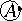
\includegraphics[scale=0.8]{chapters/080-funktionentheorie/images/operator-1.pdf}}}}

%
% Löesung linearer Differentialgleichunge mit Singularitäten
%
\subsection{Lösungen von linearen Differentialgleichungen mit Singularitäten
\label{buch:funktionentheorie:subsection:dglsing}}
Die Potenzreihenmethode hat ermöglicht, mindestens eine Lösung gewisser
linearer Differentialgleichungen zu finden.
Bei Differentialgleichungen wie der Besselschen Differentialgleichung,
deren Koeffizienten Singularitäten aufweisen, konnte aber nur eine
Lösung gefunden werden, während die Theorie verlangt, dass eine
Differentialgleichung zweiter Ordnung zwei linear unabhängige Lösungen
haben muss.

Ziel dieses Abschnitts ist zu zeigen, warum dies nicht möglich war und
wie diese Schwierigkeit mit Hilfe der analytischen Fortsetzung überwunden
werden kann.

%
% Differentialgleichungen mit Singularitäten
%
\subsubsection{Differentialgleichungen mit Singularitäten}
Mit der Besselschen
Differentialgleichung~\eqref{buch:differentialgleichungen:eqn:bessel}
ist es nicht möglich, die zweite Ableitung $y''(0)$ an der Stelle $x=0$
zu bestimmen.
Die Differentialgleichung kann an der Stelle $x=0$ nicht nach $y''$
aufgelöst werden.
Wenn man die Differentialgleichung in ein Differntialgleichungssystem
\[
\frac{d}{dx}
\begin{pmatrix}
y_1\\y_2
\end{pmatrix}
=
\begin{pmatrix}
0&1\\
1-\frac{\alpha^2}{x^2}
&
-\frac{1}{x}
\end{pmatrix}
\begin{pmatrix}
y_1\\y_2
\end{pmatrix}
\]
erster Ordnung umwandelt, zeigt sich an der Stelle $x=0$ eine
Singularität in der Matrix, die Ableitung kann also für $x=0$
nicht bestimmt werden.
In einer Umgebung von $x=0$ erfüllt die Differentialgleichung
die Voraussetzungen bekannter Existenz- und Eindeutigkeitssätze
für gewöhnliche Differentialgleichungen nicht.

Ein ähnliches Problem tritt bei jeder hypergeometrischen
Differentialgleichung auf.
Diese werden gemäss Abschnitt
\ref{buch:differentialgleichungen:section:hypergeometrisch}
aus den Differentialoperatoren
\[
D_a=z\frac{d}{dz} + a
\]
zusammengesetzt.
Die Ableitung höchster Ordnung eines Produktes solcher Operationen ist
\[
D_{a_1}
\cdots
D_{a_p}
=
z^p\frac{d^p}{dz^p} + \text{Ableitungen niedrigerer Ordnung}.
\]
Dies zeigt, dass für $p>0$ oder $q>0$ ein Faktor $x$ bei der
Ableitung höchster Ordnung unvermeidlich ist, die Differentialgleichung
kann also wieder nicht nach dieser Ableitung aufgelöst werden und
erfüllt die Voraussetzungen der Existenz- und Eindeutigkeitssätze
in einer Umgebung von $x=0$ wieder nicht.

Die Besselsche Differentialgleichung
hat auch nicht die Form $y''+p(x)xy'+q(x)=0$, die der Theorie der 
Indexgleichung zugrunde lag.
\index{Besselsche Differentialgleichung}%
\index{Differentialgleichung!Besselsche}%
Daher kann es auch keine Garantie geben, dass die Methode der
verallgemeinerten Potenzreihen zwei linear unabhängige Lösungen
liefern kann.
Tatsächlich wurde für ganzzahlige $n$ wegen $J_n(x) = (-1)^n J_{-n}(x)$
nur eine Lösung statt der erwarteten zwei linear unabhängigen
Lösungen gefunden.

Sind die Koeffizienten einer linearen Differentialgleichungen wie
in den genannten Beispielen singulär bei $x=0$, kann man auch nicht
erwarten, dass die Lösungen singulär sind.
Dies war schliesslich die Motivation, einen Lösungsansatz mit einer
verallgemeinerten Potenzreihe zu versuchen.
Mit den Funktion $x^\varrho$ lässt sich bereits eine recht grosse
Klasse von Singularitäten beschreiben, aber es ist nicht klar,
welche weiteren Arten von Singularitäten berücksichtigt werden sollten.
Dies soll im Folgenden geklärt werden.

%
% Der Lösungsraum einer Differentialgleichung zweiter Ordnung
%
\subsubsection{Der Lösungsraum einer Differentialgleichung zweiter Ordnung}
Eine Differentialgleichung $n$-ter Ordnung hat lokal einen $n$-dimensionalen
Vektorraum als Lösungsraum.

\begin{definition}
\label{buch:funktionentheorie:singularitaeten:def:loesungsraum}
Sei 
\begin{equation}
\sum_{k=0}^n a_k(x) y^{(n)}(x) = 0
\label{buch:funktionentheorie:singularitaeten:eqn:defdgl}
\end{equation}
eine Differentialgleichung $n$-ter Ordnung mit analytischen Koeffizienten
und $x_0\in \mathbb{C}$.
Dann ist
\[
\mathbb{L}_{x_0}
=
\left\{
y(x)
\;\left|\;
\begin{minipage}{6cm}
$y$ ist Lösung der Differentialgleichung
\eqref{buch:funktionentheorie:singularitaeten:eqn:defdgl}
in einer Umgebung von $x_0$
\end{minipage}
\right.
\right\}
\]
der Lösungsraum der Differentialgleichung
\eqref{buch:funktionentheorie:singularitaeten:eqn:defdgl}.
Wenn der Punkt $x_0$ aus dem Kontext klar ist, kann er auch weggelassen
werden: $\mathbb{L}_{x_0}=\mathbb{L}$.
\index{Lösungsraum einer Differentialgleichung}%
\index{Differentialgleichung!Lösungsraum}%
\end{definition}

%
% Analytische Fortsetzung auf dem Weg um 0
%
\subsubsection{Analytische Fortsetzung auf einem Weg um $0$}
Die betrachteten Differentialgleichungen haben holomorphe
Koeffizienten, Lösungen der Differentialgleichung lassen sich
daher immer in die komplexe Ebene fortsetzen, solange man die
Singularitäten der Koeffizienten vermeidet.
Hat eine Funktion $y(z)$ eine Laurent-Reihe
\[
y(z) = \sum_{k=-\infty}^\infty a_kz^k,
\]
dann ist sie automatisch in einer Umgebung von $0$ definiert
ausser in $0$.
Die analytische Fortsetzung entlang eines Pfades, der $0$
umschliesst, ist die Funktion $y(z)$ selbst.

Für die Wurzelfunktion $y(z)=z^{\frac1n}$ ist dies nicht möglich.
Die analytische Fortsetzung von $\sqrt[n]{x}$ auf der positiven reellen
Achse entlang einer Kurve, die $0$ umschliesst,
produziert die Funktion
\[
\sqrt[n]{z}
=
\sqrt[n]{re^{i\varphi}}
=
\sqrt[n]{r}e^{i\frac{\varphi}n},
\]
die für $\varphi=2\pi$ zu $e^{i\frac{2\pi}n}\sqrt{x}$ wird.
Verallgemeinerte Potenzreihen als Lösungen zeigen daher, dass
die analytische Fortsetzung der Lösung entlang eines Pfades um
eine Singularität nicht mit der Lösung übereinstimmen muss.
Das Studium dieser analytischen Fortsetzung dürfte daher zusätzliche
Informationen über die Lösung hervorbringen.

\begin{definition}
\label{buch:funktionentheorie:def:fortsetzungsoperator}
\index{Fortsetzungsoperator}%
Der {\em Fortsetzungsoperator} $\sk$ ist der lineare Operator, der eine
in einem Punkt $x\in\mathbb{R}^+$ analytische Funktion $f(x)$ entlang eines
geschlossenen Weges fortsetzt, der $0$ im Gegenuhrzeigersinn umläuft.
Die Einschränkung der analytischen Fortsetzung auf $\mathbb{R}^+$ wird
mit $\sk f(x)$ bezeichnet.
\index{analytische Fortsetzung}%
\index{Fortsetzung, analytisch}%
\end{definition}

Die obengenannten Beispiele lassen sich mit dem Operator $\sk$ als
\[
\begin{aligned}
\sk z^n
&=
z^n
&\qquad& n \in \mathbb{Z}
\\
\sk
\sum_{k=-\infty}^\infty a_kz^k
&=
\sum_{k=-\infty}^\infty a_kz^k
\\
\sk z^\varrho
&=
e^{2\pi i\varrho} z^\varrho
\end{aligned}
\]
schreiben.

%
% Rechenregeln für die analytische Fortsetzung
%
\subsubsection{Rechenregeln für die analytische Fortsetzung}
Der Operator $\sk$ ist ein Algebrahomomorphismus, d.~h.~für zwei analytische
Funktionen $f$ und $g$ gilt
\[
\begin{aligned}
\sk(\lambda f + \mu g)
&=
\lambda \sk f  + \mu \sk g
\\
\sk(fg)
&=
(\sk f)(\sk g)
\end{aligned}
\]
für beliebige $\lambda,\mu\in\mathbb{C}$.
Ist $f$ eine in ganz $\mathbb{C}$ holomorphe Funktion, dann lässt sie
sich mit Hilfe einer Potenzreihe berechnen.
Der Wert $f(g(z))$ entsteht durch Einsetzen von $g(z)$ in die Potenzreihe.
Analytische Fortsetzung mit $\sk$ reproduziert jeden einzelnen Term
der Potenzreihe, es folgt
$\sk f(g(z)) = f(\sk g(z))$.
Ebenso folgt auch, dass der Operator $\sk$ mit der Ableitung
vertauscht, dass also
\[
\frac{d^n}{dz^n}(\sk f)
=
\sk(f^{(n)}).
\]

%
% Analytische Fortsetzung von Lösungen einer Differentialgleichung
%
\subsubsection{Analytische Fortsetzung von Lösungen einer Differentialgleichung}
Wir untersuchen jetzt die Wirkung des Operators $\sk$ auf
den Lösungsraum $\mathbb{L}$ einer Differentialgleichung mit
analytischen Koeffizienten, die in einer Umgebung von $0$
definiert sind.
Auf den Koeffizienten wirkt $\sk$ als die Identität. 
Ist $y(x)$ eine Lösung der Differentialgleichung, dann gilt
\[
0
=
\sk\biggl(
\sum_{k=0}^n a_k(x) y^{(n)}(x)
\biggr)
=
\sum_{k=0}^n (\sk a_k)(x) \cdot (\sk y)^{(n)}(x)
=
\sum_{k=0}^n a_k(x) \cdot (\sk y)^{(n)}(x),
\]
somit ist $\sk y$ ebenfalls eine Lösung.
Wir schliessen daraus, dass $\sk$ eine lineare Abbildung 
$\mathbb{L}\to\mathbb{L}$ ist.

Der Lösungsraum einer Differentialgleichung $n$-ter Ordnung
ist $n$-dimensional.
Nach Wahl einer Basis des Lösungsraums kann der Operator $\sk$
mit Hilfe einer Matrix $A\in M_{n\times n}(\mathbb{C})$ beschrieben werden.
Sei $\mathscr{W}=\{w_1,\dots,w_n\}$ eine Basis des Lösungsraums, dann
kann $\sk w_j$ wieder eine Lösung der Differentialgleichung
und kann daher geschrieben werden als Linearkombination
\begin{equation}
\sk w_j
=
\sum_{k=1}^n
a_{jk} w_k
\end{equation}
der Funktionen in $\mathscr{W}$.

Die Matrix $A$ mit den Einträgen $a_{jk}$ kann durch Wahl einer
geeigneten Basis in besonders einfache Form gebracht.
Wir führen diese Diskussion im folgenden nur für eine Differentialgleichung
zweiter Ordnung $n=2$.

%
% Fall A diagonalisierbar
%
\subsubsection{Fall $A$ diagonalisierbar: verallgemeinerte Potenzreihen}
In diesem Fall kann man die Lösungsfunktionen $w_1$ und $w_2$ so
wählen, dass die Matrix
\[
A=\begin{pmatrix}\lambda_1&0\\0&\lambda_2\end{pmatrix}
\]
diagonal wird mit Eigenwerten $\lambda_j$, $j=1,2$.
Dies bedeutet, dass $\sk w_j = \lambda_j w_j$.
Wir schreiben
\[
\varrho_j = \frac{1}{2\pi i} \log\lambda_j.
\]
Der Logarithmus ist nicht eindeutig, er ist nur bis auf ein Vielfaches
von $2\pi i$ bestimmt.
Folglich aus auch $\varrho_j$ nicht eindeutig bestimmt, eine
andere Wahl des Logarithmus ändert $\varrho_j$ aber um eine ganze Zahl.

Die Funktion $z^{\varrho_j}$ wird unter der Wirkung von $\sk$ zu
\[
\sk z^{\varrho_j}
=
e^{2\pi i\varrho_j} z^{\varrho_j}
=
e^{\log \lambda_j} z^{\varrho_j}
=
\lambda_j z^{\varrho_j}.
\]
Auf den Funktionen $z^{\varrho_j}$ und $w_j$ wirkt der Operator $\sk$
also die gleich durch Multiplikation mit $\lambda_j$.
Deren Quotient
\[
f(z) = \frac{w_j(z)}{z^{\varrho_j}}
\qquad\text{erfüllt}\qquad
\sk f
=
\frac{\sk w_j}{\sk z^{\varrho_j}}
=
\frac{\lambda_j w_j}{\lambda_j z^{\varrho_j}}
=
\frac{w_j}{z^{\varrho_j}}
=
f.
\]
Die Funktion $f$ kann daher als Laurent-Reihe
\[
f(z) 
=
\sum_{k=-\infty}^\infty a_kz^k
\]
geschrieben werden.
Die Lösung $w_2(z)$ muss daher die Form
\begin{equation}
w_j(z)
=
z^{\varrho_j} f(z)
=
z^{\varrho_j} \sum_{k=-\infty}^\infty a_kz^k
\end{equation}
haben, also die einer verallgemeinerten Potenzreihe.
Auch hier zeigt sich, dass die Wahl des Logarithmus in der Definition
von $\varrho_j$ unbedeutend ist, sie äussert sich nur in einer
Verschiebung der Koeffizienten $a_k$.

Falls der Operator $\sk$ also diagonalisierbar ist, dann gibt es
zwei linear unabhängige Lösungen der Differentialgleichung in der
Form einer verallgemeinerten Potenzreihe.

%
% Fall $A$ nicht diagonalisierbar
%
\subsubsection{Fall $A$ nicht diagonalisierbar: logarithmische Lösungen}
Falls die Matrix $A$ nicht diagonalisierbar ist, hat sie nur einen
Eigenwert $\lambda$ und kann durch geeignete Wahl einer Basis in
Jordansche Normalform
\[
A
=
\begin{pmatrix}
\lambda &    1    \\
   0    & \lambda
\end{pmatrix}
\]
gebracht werden.
Dies bedeutet, dass
\begin{align*}
\sk w_1 &= \lambda w_1 + w_2
\\
\sk w_2 &= \lambda w_2.
\end{align*}
Die Funktion $w_2$ hat unter $\sk$ die gleichen Eigenschaften
wie im diagonalisierbaren Fall, man kann also wieder schliessen,
dass $w_2$ durch eine verallgemeinerte Potenzreihe mit
\[
\varrho=\frac{1}{2\pi i} \log \lambda
\]
dargestellt werden kann.

Für den Quotienten $w_1/w_2$ findet man jetzt das Bild
\begin{equation}
\sk \frac{w_1}{w_2}
=
\frac{\sk w_1}{\sk w_2}
=
\frac{\lambda w_1+w_2}{\lambda w_2}
=
\frac{w_1}{w_2} + \frac{1}{\lambda}
\label{buch:funktionentheorie:singularitaeten:sklog}
\end{equation}
Das Verhalten von $w_1$ unter $\sk$ in
\eqref{buch:funktionentheorie:singularitaeten:sklog}
ist dasselbe wie bei $\log(z)/\lambda$, denn
\[
\sk \frac{\log(z)}{\lambda}
=
\frac{\log(z)}{\lambda} + 1.
\]
Die Differenz $w_1-\log(z)/\lambda$ wird bei der analytischen
Fortsetzung zu
\[
\sk\biggl(
\frac{w_1}{w_2}-\frac{\log(z)}{\lambda}
\biggr)
=
\sk \frac{w_1}{w_2} - \sk\frac{\log(z)}{\lambda}
=
\frac{w_1}{w_2} + \frac{1}{\lambda}
-
\frac{\log(z)}{\lambda}
-\frac{1}{\lambda}
=
\frac{w_1}{w_2}-\frac{\log(z)}{\lambda}.
\]
Die Differenz ist daher wieder als Laurent-Reihe
\[
\frac{w_1}{w_2}-\frac{\log(z)}{\lambda}
=
\sum_{k=-\infty}^\infty b_kz^k
\]
darstellbar, was nach $w_1$ aufgelöst 
\[
w_1(z)
=
\frac{1}{\lambda} \log(z) w_2(z)
+
w_2(z) \sum_{k=-\infty}^\infty b_kz^k
\]
ergibt.
Da $w_2$ eine verallgemeinerte Potenzreihe ist, kann man dies auch
als
\begin{equation}
w_1(z)
=
c \log(z) w_2(z)
+
z^{\varrho}
\sum_{k=-\infty}^{\infty} c_kz^k
\label{buch:funktionentheorie:singularitäten:eqn:w1}
\end{equation}
schreiben, wobei Konstanten $c$ und $c_k$ noch bestimmt werden müssen.
Setzt man
\eqref{buch:funktionentheorie:singularitäten:eqn:w1}
in die ursprüngliche Differentialgleichung ein, verschwindet der
$\log(z)$-Term und für die verbleibenden Koeffizienten kann die
bekannte Methode des Koeffizientenvergleichs verwendet werden.

%
% Bessel-Funktionen zweiter Art
%
\subsubsection{Bessel-Funktionen zweiter Art
\label{buch:funktionentheorie:subsubsection:bessel2art}}
Im Abschnitt~\ref{buch:differentialgleichungen:subsection:bessel1steart}
waren wir nicht in der Lage, für ganzahlige $\alpha$ zwei linear unabhängige
Lösungen der Besselschen Differentialgleichung zu finden.
Die vorangegangenen Ausführungen erklären dies: der Ansatz als
verallgemeinerte Potenzreihe konnte die Singularität nicht wiedergeben.
Inzwischen wissen wir, dass wir nach einer Lösung mit einer logarithmischen
Singularität suchen müssen.

Um dies nachzuprüfen, setzen wir den Ansatz
\[
y(x) = \log(x) J_n(x) + z(x)
\]
in die Besselsche Differentialgleichung ein.
Dazu benötigen wir erst die Ableitungen von $y(x)$:
\begin{align*}
y'(x)
&=
\frac{1}{x} J_n(x) + \log(x)J_n'(x) + z'(x)
\\
xy'(x)
&=
J_n(x) + x\log(x)J_n'(x) + xz'(x)
\\
y''(x)
&=
-\frac{1}{x^2} J_n(x)
+\frac2x J_n'(x)
+\log(x) J_n''(x)
+z''(x)
\\
x^2y''(x)
&=
-J_n(x) + 2xJ'_n(x)+x^2\log(x)J_n''(x) + x^2z''(x).
\end{align*}
Die Wirkung des Bessel-Operators auf $y(x)$ ist
\begin{align*}
By
&=
x^2y''+xy'+x^2y
\\
&=
\log(x) \bigl(
\underbrace{
x^2J_n''(x)
+xJ_n'(x)
+x^2J_n(x)
}_{\displaystyle = n^2J_n(x)}
\bigr)
-J_n(x)+2xJ_n'(x)
+J_n(x)
+
xz'(x)
+
x^2z''(x)
\\
&=
n^2 \log(x)J_n(x)
+
2xJ_n(x)
+
x^2z(x)
+
xz'(x)
+
x^2z''(x)
\end{align*}
Damit $y(x)$ eine Eigenfunktion zum Eigenwert $n^2$ wird, muss 
dies mit $n^2y(x)$ übereinstimmen, also
\begin{align*}
n^2 \log(x)J_n(x)
+
2xJ_n(x)
+
x^2z(x)
+
xz'(x)
+
x^2z''(x)
&=
n^2\log(x)J_n(x) + n^2z(x).
\intertext{Die logarithmischen Terme heben sich weg und es bleibt}
x^2z''(x)
+
xz'(x)
+
(x^2-n^2)z(x)
&=
-2xJ_n(x).
\end{align*}
Eine Lösung für $z(x)$ kann mit Hilfe eines Potenzreihenansatzes
gefunden werden.
Sie ist aber nur bis auf einen Faktor festgelegt.
Tatsächlich kann man aber auch eine direkte Definition geben.

\begin{definition}
Die Bessel-Funktionen zweiter Art der Ordnung $\alpha$ sind die Funktionen
\begin{equation}
Y_\alpha(x)
=
\frac{J_\alpha(x) \cos \alpha\pi  - J_{-\alpha}(x)}{\sin \alpha\pi }.
\label{buch:funktionentheorie:bessel:2teart}
\end{equation}
Für ganzzahliges $\alpha$ verschwindet der Nenner in 
\eqref{buch:funktionentheorie:bessel:2teart},
daher ist
\[
Y_n(x)
=
\lim_{\alpha\to n} Y_{\alpha}(x)
=
\frac{1}{\pi}\biggl(
\frac{d}{d\alpha}J_{\alpha}(x)\bigg|_{\alpha=n}
+
(-1)^n
\frac{d}{d\alpha}J_{\alpha}(x)\bigg|_{\alpha=-n}
\biggr).
\]
\end{definition}

Die Funktionen $Y_\alpha(x)$ sind Linearkombinationen der Lösungen
$J_\alpha(x)$ und $J_{-\alpha}(x)$ und damit automatisch auch Lösungen
der Besselschen Differentialgleichung.
Dies gilt auch für den Grenzwert im Falle ganzahliger Ordnung $\alpha$.
Da $J_{\alpha}(x)$ durch eine Reihenentwicklung definiert ist, kann man
diese Termweise nach $\alpha$ ableiten und damit auch eine 
Reihendarstellung von $Y_n(x)$ finden.
Nach einiger Rechnung findet man:
\begin{align*}
Y_n(x)
&=
\frac{2}{\pi}J_n(x)\log\frac{x}2
-
\frac1{\pi}
\sum_{k=0}^{n-1} \frac{(n-k-1)!}{k!}\biggl(\frac{x}2\biggr)^{2k-n}
\\
&\qquad\qquad
-
\frac1{\pi}
\sum_{k=0}^\infty \frac{(-1)^k}{k!\,(n+k)!}
\biggl(
\frac{\Gamma'(n+k+1)}{\Gamma(n+k+1)}
+
\frac{\Gamma'(k+1)}{\Gamma(k+1)}
\biggr)
\biggl(
\frac{x}2
\biggr)^{2k+n}
\end{align*}
(siehe auch \cite[p.~200]{buch:specialfunctions}).

